\documentclass{standalone}
\usepackage{xcolor}
\usepackage{tikz}
\usetikzlibrary{positioning, shapes.multipart, calc, graphs, graphs.standard}
\begin{document}
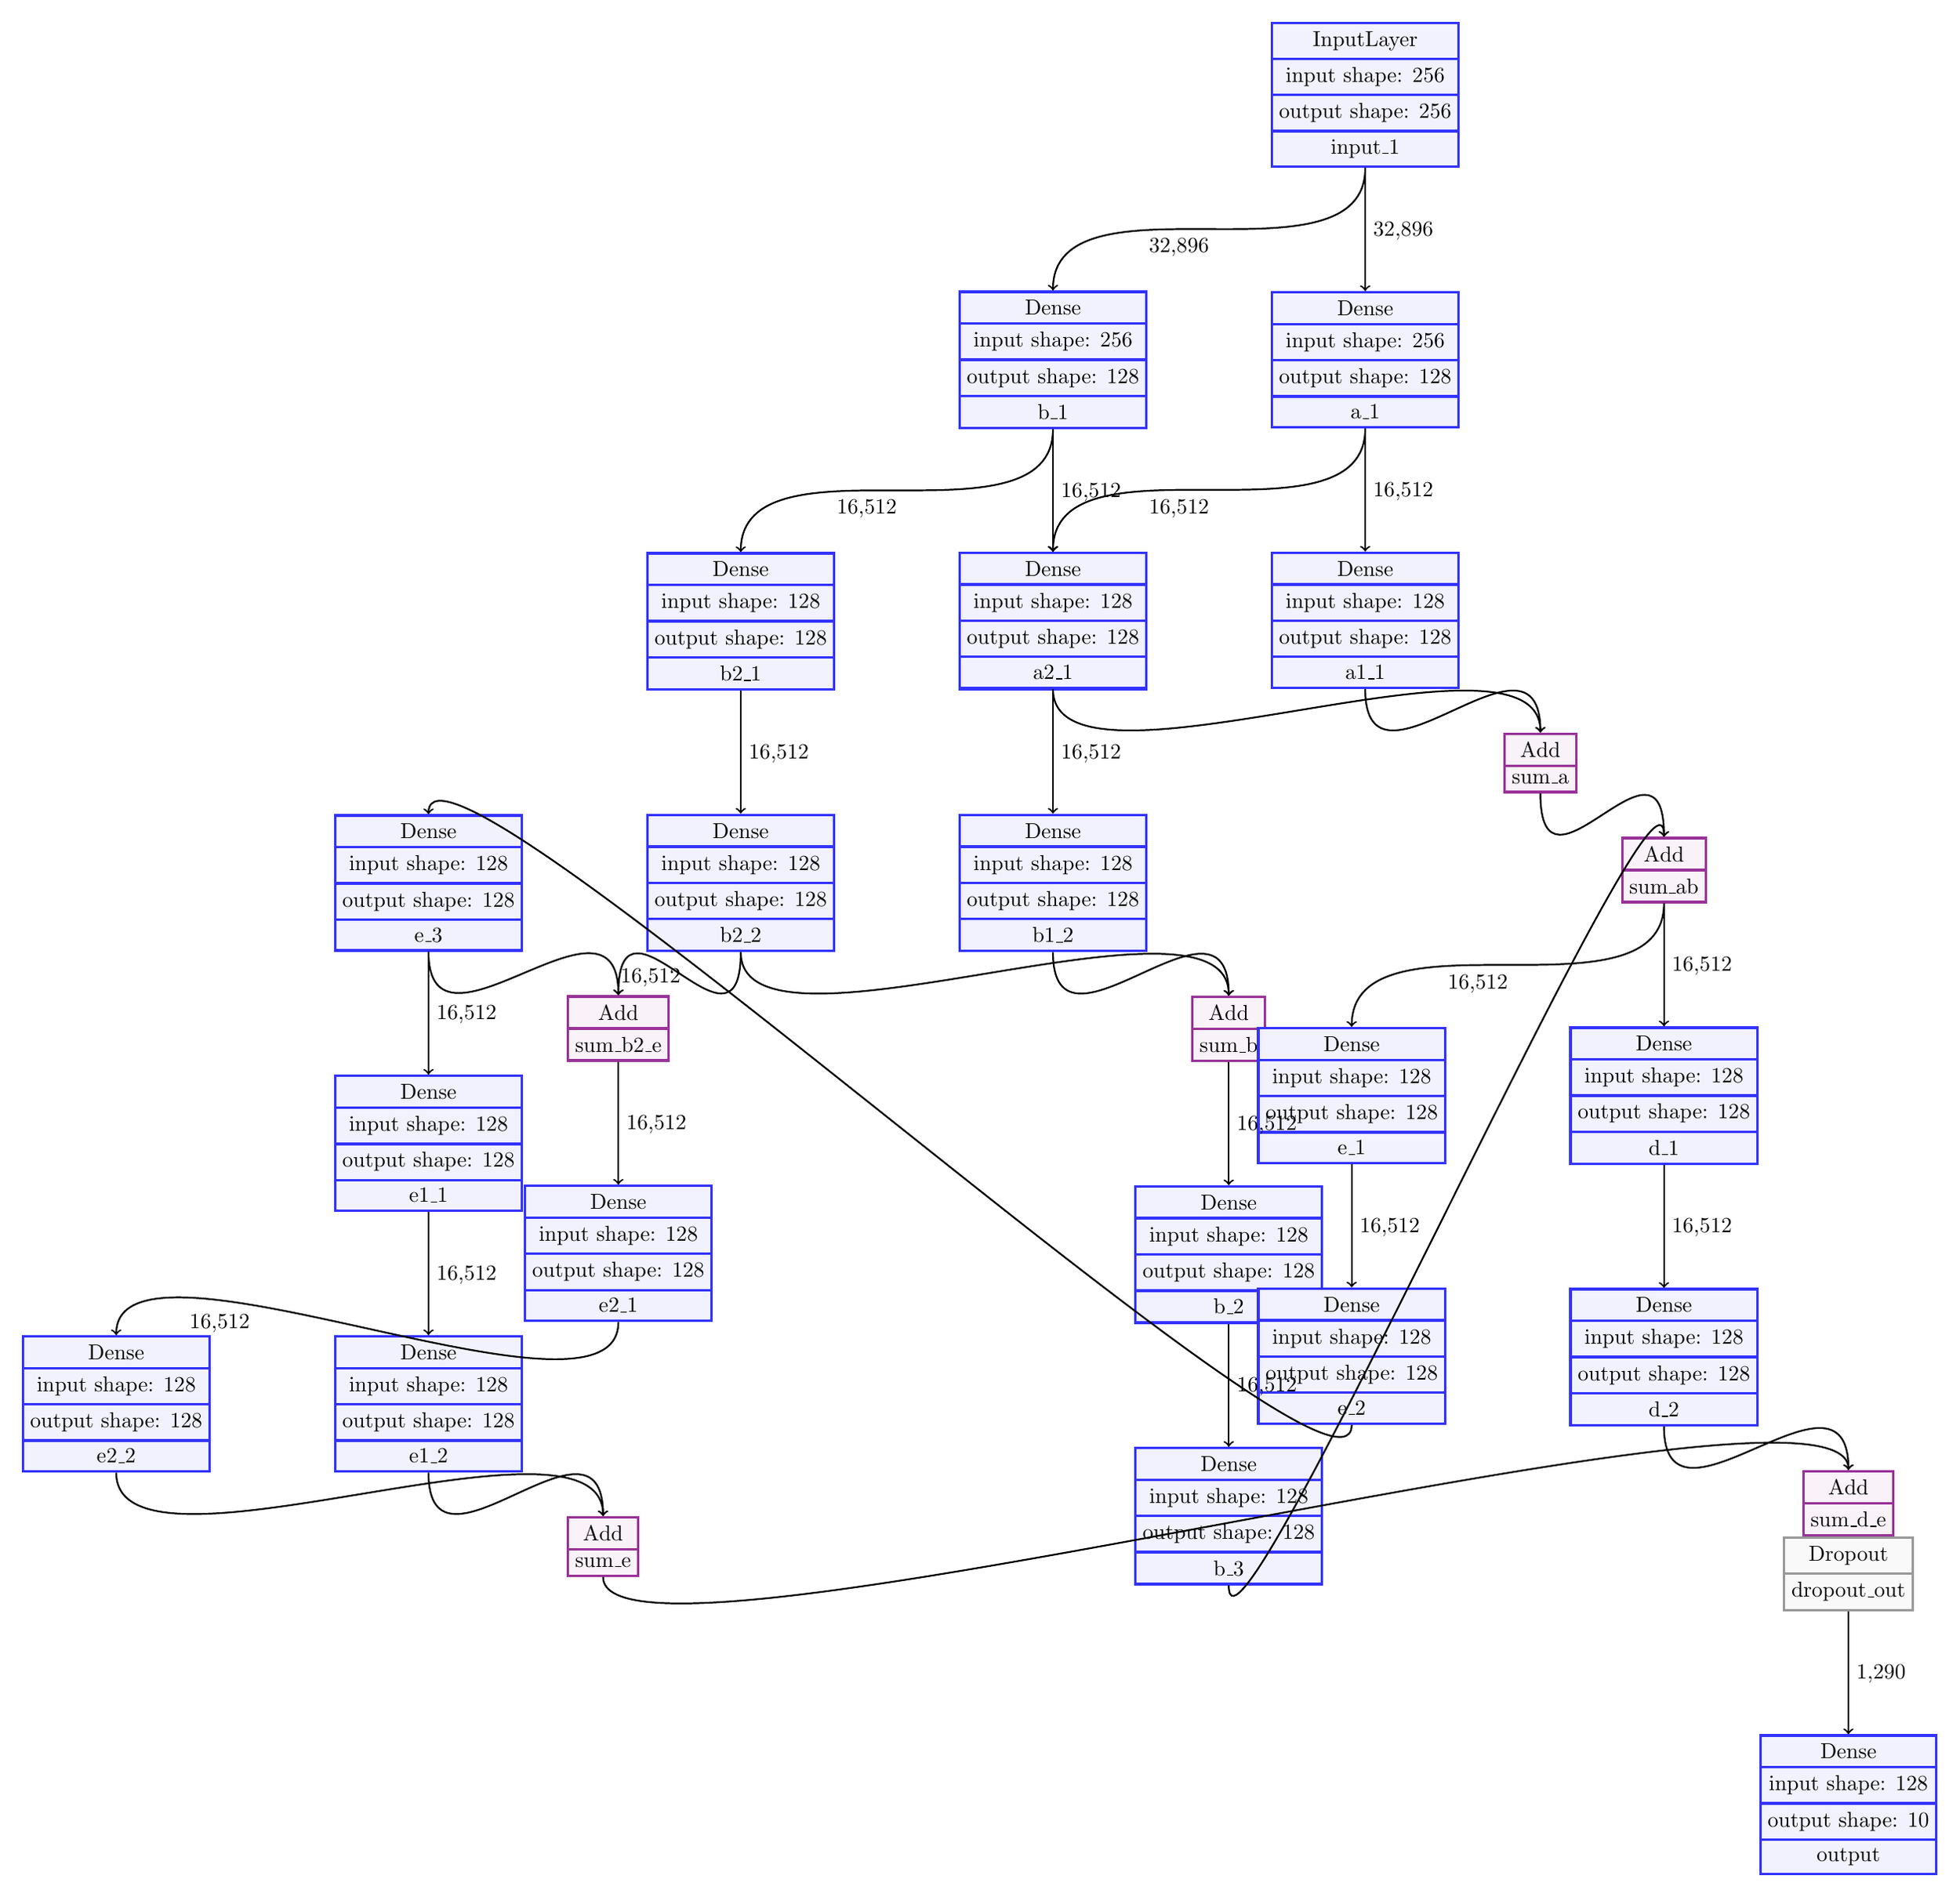
\begin{tikzpicture}
[default_edge/.style={thick,out=-90,in=90,out distance=2cm,in distance=2cm},default_label/.style={auto,pos=0.65},TrainableLayer_style/.style={rectangle split,rectangle split ignore empty parts,very thick,node distance=2cm,draw=blue!80,fill=blue!5},OperationLayer_style/.style={rectangle split,rectangle split ignore empty parts,very thick,node distance=1cm,draw=violet!80,fill=violet!5},UtilityLayer_style/.style={rectangle split,rectangle split ignore empty parts,very thick,node distance=0cm,draw=gray!80,fill=gray!5}]
\node[TrainableLayer_style] [] (input_1) {\nodepart{one}{InputLayer}\nodepart{two}{input shape: 256}\nodepart{three}{output shape: 256}\nodepart{four}{input\_1}};
\node[TrainableLayer_style] [below=of input_1] (a_1) {\nodepart{one}{Dense}\nodepart{two}{input shape: 256}\nodepart{three}{output shape: 128}\nodepart{four}{a\_1}};
\node[TrainableLayer_style] [below=of input_1,left=of a_1] (b_1) {\nodepart{one}{Dense}\nodepart{two}{input shape: 256}\nodepart{three}{output shape: 128}\nodepart{four}{b\_1}};
\node[TrainableLayer_style] [below=of b_1] (b1_1) {\nodepart{one}{Dense}\nodepart{two}{input shape: 128}\nodepart{three}{output shape: 128}\nodepart{four}{b1\_1}};
\node[TrainableLayer_style] [below=of b1_1] (b1_2) {\nodepart{one}{Dense}\nodepart{two}{input shape: 128}\nodepart{three}{output shape: 128}\nodepart{four}{b1\_2}};
\node[TrainableLayer_style] [below=of a_1] (a1_1) {\nodepart{one}{Dense}\nodepart{two}{input shape: 128}\nodepart{three}{output shape: 128}\nodepart{four}{a1\_1}};
\node[TrainableLayer_style] [below=of b_1,left=of b1_1] (b2_1) {\nodepart{one}{Dense}\nodepart{two}{input shape: 128}\nodepart{three}{output shape: 128}\nodepart{four}{b2\_1}};
\node[TrainableLayer_style] [below=of a_1,left=of a1_1] (a2_1) {\nodepart{one}{Dense}\nodepart{two}{input shape: 128}\nodepart{three}{output shape: 128}\nodepart{four}{a2\_1}};
\node[TrainableLayer_style] [below=of b2_1,left=of b1_2] (b2_2) {\nodepart{one}{Dense}\nodepart{two}{input shape: 128}\nodepart{three}{output shape: 128}\nodepart{four}{b2\_2}};
\node[OperationLayer_style] [below right=of b1_2] (sum_b) {\nodepart{one}{Add}\nodepart{two}{sum\_b}};
\node[OperationLayer_style] [below right=of a1_1] (sum_a) {\nodepart{one}{Add}\nodepart{two}{sum\_a}};
\node[TrainableLayer_style] [below=of sum_b] (b_2) {\nodepart{one}{Dense}\nodepart{two}{input shape: 128}\nodepart{three}{output shape: 128}\nodepart{four}{b\_2}};
\node[TrainableLayer_style] [below=of b_2] (b_3) {\nodepart{one}{Dense}\nodepart{two}{input shape: 128}\nodepart{three}{output shape: 128}\nodepart{four}{b\_3}};
\node[OperationLayer_style] [below right=of sum_a] (sum_ab) {\nodepart{one}{Add}\nodepart{two}{sum\_ab}};
\node[TrainableLayer_style] [below=of sum_ab] (d_1) {\nodepart{one}{Dense}\nodepart{two}{input shape: 128}\nodepart{three}{output shape: 128}\nodepart{four}{d\_1}};
\node[TrainableLayer_style] [below=of sum_ab,left=of d_1] (e_1) {\nodepart{one}{Dense}\nodepart{two}{input shape: 128}\nodepart{three}{output shape: 128}\nodepart{four}{e\_1}};
\node[TrainableLayer_style] [below=of e_1] (e_2) {\nodepart{one}{Dense}\nodepart{two}{input shape: 128}\nodepart{three}{output shape: 128}\nodepart{four}{e\_2}};
\node[TrainableLayer_style] [below=of e_2,left=of b2_2] (e_3) {\nodepart{one}{Dense}\nodepart{two}{input shape: 128}\nodepart{three}{output shape: 128}\nodepart{four}{e\_3}};
\node[TrainableLayer_style] [below=of e_3] (e1_1) {\nodepart{one}{Dense}\nodepart{two}{input shape: 128}\nodepart{three}{output shape: 128}\nodepart{four}{e1\_1}};
\node[TrainableLayer_style] [below=of e1_1] (e1_2) {\nodepart{one}{Dense}\nodepart{two}{input shape: 128}\nodepart{three}{output shape: 128}\nodepart{four}{e1\_2}};
\node[TrainableLayer_style] [below=of d_1] (d_2) {\nodepart{one}{Dense}\nodepart{two}{input shape: 128}\nodepart{three}{output shape: 128}\nodepart{four}{d\_2}};
\node[OperationLayer_style] [below right=of e_3] (sum_b2_e) {\nodepart{one}{Add}\nodepart{two}{sum\_b2\_e}};
\node[TrainableLayer_style] [below=of sum_b2_e] (e2_1) {\nodepart{one}{Dense}\nodepart{two}{input shape: 128}\nodepart{three}{output shape: 128}\nodepart{four}{e2\_1}};
\node[TrainableLayer_style] [below=of e2_1,left=of e1_2] (e2_2) {\nodepart{one}{Dense}\nodepart{two}{input shape: 128}\nodepart{three}{output shape: 128}\nodepart{four}{e2\_2}};
\node[OperationLayer_style] [below right=of e1_2] (sum_e) {\nodepart{one}{Add}\nodepart{two}{sum\_e}};
\node[OperationLayer_style] [below right=of d_2] (sum_d_e) {\nodepart{one}{Add}\nodepart{two}{sum\_d\_e}};
\draw[->, default_edge] (input_1) to node [default_label] {32,896} (b_1);
\node[UtilityLayer_style] [below=of sum_d_e] (dropout_out) {\nodepart{one}{Dropout}\nodepart{two}{dropout\_out}};
\draw[->, default_edge] (b_1) to node [default_label] {16,512} (b1_1);
\node[TrainableLayer_style] [below=of dropout_out] (output) {\nodepart{one}{Dense}\nodepart{two}{input shape: 128}\nodepart{three}{output shape: 10}\nodepart{four}{output}};
\draw[->, default_edge] (b_1) to node [default_label] {16,512} (b2_1);
\draw[->, default_edge] (b1_1) to node [default_label] {16,512} (b1_2);
\draw[->, default_edge] (b2_1) to node [default_label] {16,512} (b2_2);
\draw[->, default_edge] (input_1) to node [default_label] {32,896} (a_1);
\draw[->, default_edge] (b1_2) to node [default_label] {} (sum_b);
\draw[->, default_edge] (b2_2) to node [default_label] {} (sum_b);
\draw[->, default_edge] (a_1) to node [default_label] {16,512} (a1_1);
\draw[->, default_edge] (a_1) to node [default_label] {16,512} (a2_1);
\draw[->, default_edge] (sum_b) to node [default_label] {16,512} (b_2);
\draw[->, default_edge] (a1_1) to node [default_label] {} (sum_a);
\draw[->, default_edge] (a2_1) to node [default_label] {} (sum_a);
\draw[->, default_edge] (b_2) to node [default_label] {16,512} (b_3);
\draw[->, default_edge] (sum_a) to node [default_label] {} (sum_ab);
\draw[->, default_edge] (b_3) to node [default_label] {} (sum_ab);
\draw[->, default_edge] (sum_ab) to node [default_label] {16,512} (e_1);
\draw[->, default_edge] (e_1) to node [default_label] {16,512} (e_2);
\draw[->, default_edge] (e_2) to node [default_label] {16,512} (e_3);
\draw[->, default_edge] (e_3) to node [default_label] {} (sum_b2_e);
\draw[->, default_edge] (b2_2) to node [default_label] {} (sum_b2_e);
\draw[->, default_edge] (e_3) to node [default_label] {16,512} (e1_1);
\draw[->, default_edge] (sum_b2_e) to node [default_label] {16,512} (e2_1);
\draw[->, default_edge] (sum_ab) to node [default_label] {16,512} (d_1);
\draw[->, default_edge] (e1_1) to node [default_label] {16,512} (e1_2);
\draw[->, default_edge] (e2_1) to node [default_label] {16,512} (e2_2);
\draw[->, default_edge] (d_1) to node [default_label] {16,512} (d_2);
\draw[->, default_edge] (e1_2) to node [default_label] {} (sum_e);
\draw[->, default_edge] (e2_2) to node [default_label] {} (sum_e);
\draw[->, default_edge] (d_2) to node [default_label] {} (sum_d_e);
\draw[->, default_edge] (sum_e) to node [default_label] {} (sum_d_e);
\draw[->, default_edge] (dropout_out) to node [default_label] {1,290} (output);
\end{tikzpicture}\end{document}